\documentclass[a4paper,12pt]{article}
\usepackage[utf8]{inputenc}
\usepackage[final]{neurips_2018}
\usepackage{amsmath}
\usepackage{algorithm}
\usepackage[noend]{algpseudocode}
\usepackage{graphicx}

%opening
\title{Online influence maximization with different propagation models}
\author{Paul Chevalier, Tangi Hetet\\[0.5cm]{Supervisor: Pierre Perrault}}

\begin{document}

\maketitle

\begin{abstract}
\begin{center}
 \textbf{Need to write it at the end }
\end{center}
\end{abstract}

\section{Introduction}
\label{scn:intro}

\subsection{Motivation}

The study of social networks play an important role in understanding the spread of ideas, technologies and influence among its members, and has a lot of practical and commercial applications. The underlying idea behind the concept of influence maximization is that an idea circulating through a social network can either die out or spread rapidly, depending on the influence people can have on their peers, and the extent to which they are affected by their decisions. Thus, the underlying problem posed is to choose where to implant an idea in a social network to maximize the idea's propagation. This problem is named \emph{social influence maximization}, and has a lot of practical applications, including innovation propagation~\cite{coleman1966medical}, viral marketing~\cite{bass1976new}, etc.

There are several formulations of the problem, depending on the amount of information the player has. However, the optimal solution for this problem is NP-hard for most models that have been studied, notably the model in ~\cite{domingos2001mining}. For this reason, most studies in literature insists on finding approximate solutions to the problem.

\subsection{Previous work}

We study some of the work that has been done on this subject. Note that in our setting, the influence between nodes of the social network is unknown, and therefore our problem can be seen as an example of a bandit problem.

\subsubsection{Multi-Armed Bandit}

In probability theory, the multi-armed bandit problem is a classic reinforcement learning problem that exemplifies the exploration-exploitation tradeoff dilemna, where the player has to maximize its gain over an environment he only has partial knowledge about. At each round, the player chooses an arm and pulls it, and the environment rewards the player. The player then uses the feedback he gets to improve his estimate of the average reward of the arm he just pulled.

Notably, one of the proposed approach to this problem is the \emph{Upper Confidence Bound} algorithm (UCB)~\cite{li2010contextual}. This algorithm consists in adding to the estimated mean of each arm a confidence bound, corresponding to an optimism bonus towards uncertainty, and then choose the arm with the best score. This allows to perform exploration of the arms that have not been used a lot yet.

Another known approach is the Thompson sampling algorithm~\cite{thompson1933likelihood}, which uses a bayesian approach to estimate the average rewards of the arms.

There exist many variants of the classical MAB problem. Particularly, we focus here on CMAB and CMAB-T variants. CMAB, or \emph{Combinatorial Multi-Armed Bandit}, differs from the classical MAB setting in that there is not a single triggered arm at each round, but a set of arms. The player chooses an action, which correspond to triggering several arms at a time. He thus get a wider feedback about the arms. Another variant, denoted as CMAB-T corresponds to the CMAB setting, except that a given action can trigger arms probabilistically. Thus, some arms may be difficult to trigger.


\subsubsection{Influence maximization}

Social influence maximization was first modeled as an algorithmic problem by Kempe et al.~\cite{kempe2003maximizing}. Due to the intrinsic complexity of the problem, most works consist in finding appproximate solution. Kempe et al.~\cite{kempe2003maximizing} proposed a simple and efficient greedy algorithm that allows to get a $(1-1/e-\epsilon)$ approximation of the solution, however it is computationnaly expensive. In particular, it has $\Omega(k\cdot|V|\cdot|E|\cdot\text{Poly}(1/\epsilon))$ time complexity, which makes it unusable on large graphs. A significant improvement was done by Borgs et al.~\cite{borgs2014maximizing}, who proposed an algorithm that yields an $(1-1/e-\epsilon)$-approximate solution with probability at least $1-n^{-l}$ probability, and with a time complexity of $O(kl^2(m+n)\log^2 n / \epsilon^3)$. Although this method is theoretically near-optimal, since any other algorithm that provides the same approximation guarantee and succeeds with at least a constant probability must run in $\Omega(m + n)$ time~\cite{borgs2014maximizing}, it is practically unsatisfactory because it is very slow, due to a large hidden multiplicative constant in the runtime bound. Tang et al.~\cite{tang2014influence} proposed another algorithm, called \emph{Two-Phase Influence Maximization} (TIM), that ensures near optimal runtime $O((k + l)(n + m) \log n/\epsilon^2)$ and can be run efficiently on very large graphs.

\subsubsection{Influence maximization bandit}

The influence maximization bandit problem is pretty similar to the previous problem, except that the probability associated to the influence between nodes of the graph are not known. For this reason, the problem becomes equivalent to a bandit problem, since the player needs to estimate these probabilities while trying to maximize influence. In particular, Chen et al.~\cite{chen2016combinatorial} study this problem and derive a lower bound for the expected regret of the algorithm.

\subsection{Our work}

In this work, we study the algorithm proposed by Wang et Chen~\cite{wang2017improving} for the combinatorial semi-bandits setting to the online influence maximization problem. Since this algorithm uses an heuristics to perform the actual influence maximization, we also go into details about the choice of heuristic for this part of the optimization. We then perform some experiments on the Stanford Large Network Dataset Collection~\cite{leskovec2015snap}. In part \ref{scn:def} we formally define the problem, in part \ref{scn:algo} we describe the algorithm and the theorical guarantees associated, and in part \ref{scn:exp} we describe our experimentations.


\section{Definitions}
\label{scn:def}

In order to formally define the online influence maximization problem, we first define the Combinatorial Multi-Armed Bandit problem, which will be necessary to our definition.

\subsection{CMAB-T}

The CMAB-T problem is defined as a learning game, as follows. The environment consists of $m$ arms, described as random variables $X = (X_1, ..., X_m)$ following a joint distribution $D\in \mathcal{D}$ where $\mathcal{D}$ is a class of distributions over $[0, 1]^m$.  $D$ is fixed at the beginning of the game and unknown to the player, whereas $\mathcal{D}$ is known.

At time $t\in\mathbf{N}^*$, the player picks an action $s_t\in\mathcal{S}$ (where $\mathcal{S}$ is potentially infinite) and the environment draws a sample $x^{(t)} = (x^{(t)}_1, ..., x^{(t)}_m)$ of the variable $X$. The action $s_t$ triggers a set of arm $\tau_t$, so that the player has access to the values $(x_i)_{i\in\tau_t}$, which in turn yields a reward $R(s_t, x^{(t)}, \tau_t)$ to the player. The expected reward is assumed to be only a function of the expected value of $X$, that is if $\mu = (\mu_i)_{i\in\{1, ..., m\}} = (\mathbf{E}[X_i])_{i\in\{1, ..., m\}}$, then $\mathbf{E}[R(s_t, x^{(t)}, \tau_t)] = r_{s_t}(\mu)$.

The player has access to an offline $(\alpha, \beta)$-approximation oracle $\mathcal{O}$, which takes $\mu$ as input and outputs an action $\mathcal{S}^{\mathcal{O}}$ such that $\mathbf{P}(r_{\mathcal{S}^{\mathcal{O}}}(\mathcal{\mu}) \geq \alpha\cdot\sup_{s\in\mathcal{S}}r_S(\mu)) \geq \beta$.

The goal of the player is to maximize the reward over time, or equivalently to minimize the $(\alpha, \beta)$-regret, that is defined as the hypothetical loss due to not choosing the best action when disposing of an offline $(\alpha, \beta)$-approximation oracle: 

\begin{equation}
 \label{eqn:regret}
\text{Reg}_{\mu, \alpha, \beta}(T) = T\cdot\alpha\cdot\beta\cdot\sup_{s\in\mathcal{S}}r_S(\mu) - \mathbf{E}\left[\sum_{t = 1}^{T}r_{s^{t}}(\mu)\right]
\end{equation}

\subsection{Online influence maximization}

In social influence maximization, we are given a weighted directed graph $(V, E, p)$, where $V$ is the set of vertices of the graph, $E\subseteq V\times V$ is the set of edges and $p:E\to [0, 1]$ are the probabilities associated to the edges. We then define the \emph{spread} of a k-seed set $S$. Initially, we choose $k$ vertices, which are the active nodes. Then at each iteration, we propagate the active vertices according to the following rule. If at time $(t-1)$ the vertex $u$ was activated, at time $t$, for each out-neighbor $v$ of $u$ ($(u, v)\in E$) that is not active yet, $u$ has probability $p(u, v)$ of activating $v$. $u$ cannot activate its out-neighbors during during times $t' > t$. This process goes on until there are no new active nodes. The \emph{spread} of $S$ is the cardinality of the vertices that have been reached by this process. The influence maximization problem consists in finding the seed set $S$ that maximizes the spread.

Kempe et al.~\cite{kempe2003maximizing} showed that the process previously described is equivalent to determining once in advance a subset of edges of $E$ called \emph{live edges}, and defining the \emph{spread} of $S$ as the cardinal of the set of nodes reachable from $S$ through at least one path consisting only of live edges. In this equivalent process, to each edge $e$ is associated a random variable $X_e \in {0, 1}$ s.t. ($X_e = 1 \iff e$ is a live edge), for which $\mathbf{P}(X_e = 1) = p(e)$. The $(X_e)_{e \in E}$ are mutually independent.

A variant of this problem is the online influence maximization bandit~\cite{chen2016combinatorial}, a CMAB-T problem. In this setting, the arms are precisely the mutually independent variables $X_e \sim Bernoulli(p(e))$ for each ${e \in E}$, where the $(p(e))_{e \in E}$ are unknown to the player and need to be learned over time. At each iteration, an instance $X^{(t)}$ of the arms is drawn. Then the player chooses a seed set $S_t$, which determines a set of influenced nodes under the live edges (the $e$ s.t. $X_{e}^{(t)} = 1$). The triggered arms $\tau_t$ are all variables $X_e^{(t)}$ where $e = (i, j)$ is such that $i$ is an influenced node, and the reward is the spread of the seed set (the number of influenced nodes).



\section{Algorithm}
\label{scn:algo}

\subsection{Description}

The algorithm proposed by Wang et Chen~\cite{wang2017improving}, called CUCB, is a pretty straightforward UCB-type algorithm (see algorithm \ref{alg:cucb}), with a confidence radius $\rho_i = \sqrt{\frac{3\log t}{2T_i}}$, where $T_i$ is the number of times the arm $i$ has been pulled so far. Once the algorithm has computed the upper confidence bound $\bar{\mu}_i = \min\{\hat{\mu}_i + \rho_i, 1\}$, it uses an oracle to choose the action: the oracle is the function that picks the best action, based on the estimated upper confidence bounds. In our case, the oracle needs to predict the best seed set of $k$ nodes based on the estimated probabilities of the edges: this problem is the classical social influence maximization problem.


\begin{algorithm}
\caption{CUCB with computation oracle}\label{alg:cucb}
\hspace*{\algorithmicindent} \textbf{Input: } $m$, Oracle
\begin{algorithmic}[1]
\State For each arm $i$, $T_i = 0$ (maintain the total number of times arm $i$ is played so far)
\State For each arm $i$, $\hat{\mu}_i = 1$ (maintain the empirical mean of $X_i$)
\For {t = 1, 2, 3, ...}
\State For each arm $i\in[m]$, $\rho_i = \sqrt{\frac{3\log t}{2T_i}}$ (the confidence radius $\rho_i = +\infty$ if $T_i = 0$)
\State For each arm $i\in[m]$, $\bar{\mu}_i = \min\{\hat{\mu}_i + \rho_i, 1\}$ (the upper confidence bound)
\State $S = \text{Oracle}(\bar{\mu}_1, ..., \bar{\mu}_m)$
\State Play action $S$, which triggers a set $\tau \subseteq[m]$ of base arms with feedback $X_i^{(t)}, i\in\tau$
\State For every $i\in\tau$, update $T_i$ and $\hat{\mu}_i$: $T_i = T_i+1$, $\hat{\mu}_i = \hat{\mu}_i + (X_i^{(t)} - \hat{\mu}_i) / T_i$
\EndFor
\end{algorithmic}
\end{algorithm}

The oracle we use is the TIM+ algorithm proposed by Tang et al.~\cite{tang2014influence} (see subsection \ref{sscn:oracle} for details)

\subsection{Thompson sampling}

We also implement the Thomson sampling method~\cite{thompson1933likelihood} to compare with the result obtained with the CUCB algorithm. The pseudocode is detailed in algorithm \ref{alg:thompson}.

\begin{algorithm}
\caption{Thompson sampling with computation oracle}\label{alg:thompson}
\hspace*{\algorithmicindent} \textbf{Input: } $m$, Oracle
\begin{algorithmic}[1]
\State For each arm $i$, $S_i = 0$ (maintain the sum of rewards gathered from pulling arm $i$)
\State For each arm $i$, $N_i = 0$ (maintain the number of times the arm $i$ is pulled)
\For {$i = 1,2,3, ...$}
\State For each arm $i$, draw a mean sample $\tilde{\mu}_i \sim \text{Beta}(S_i + 1, N_i - S_i + 1)$
\State $S = \text{Oracle}(\tilde{\mu_1}, ..., \tilde{\mu}_m)$.
\State Play action $S$, which triggers a set $\tau \subseteq[m]$ of base arms with feedback $X_i^{(t)}, i\in\tau$
\State For each arm $i\in\tau$, update $S_i = S_i + X_i^{(t)}$ and $N_i = N_i + 1$.
\EndFor
\end{algorithmic}
\end{algorithm}

\subsection{Regret bound}

The authors prove a regret bound under the following conditions: 
\paragraph{Condition 1: monotonicity}
We say that a CMAB-T problem instance satisfies monotonicity, if for any action $S\in\mathcal{S}$, for any two distributions $D, D'\in\mathcal{D}$ with expectation vectors $\mu = (\mu_1, ..., \mu_m)$, and $\mu' = (\mu_1', ..., \mu_m')$, we have $r_S(\mu) \leq r_S(\mu')$ if $\forall i, \mu_i\leq \mu_i'$

\paragraph{Condition 2: TPM}
We say that a CMAB-T problem instance satisfies 1-norm TPM bounded smoothness, if there exists $B\in\mathbf{R}^+$ s.t. for any two distributions $D, D'\in\mathcal{D}$ with expectation vectors $\mu$ and $\mu'$, and any action $S$, we have $|r_S(\mu)-r_S(\mu')| \leq B\sum_{i\in[m]}p_i^{D,S} |\mu_i-\mu_i'|$, where $p_i^{D, S}$ is the probability that action $S$ triggers arm $i$ when the environment instance is $D$.

The first condition indicates that an increase of $\mu$ implies an increase in the reward, which is important to make the feedback we get on the arms useful to improve the reward. The second condition corresponds to a generalization of the linear condition used in linear bandits~\cite{kveton2015tight}.

\paragraph{Theorem: regret bound}
For the CUCB algorithm on a CMAB-T problem instance that satisfies monotonicity (condition 1) and 1-norm TPM bounded smoothness (condition 2), the $(\alpha, \beta)$-regret satisfies:
\begin{equation}
 \text{Reg}_{\mu, \alpha, \beta}(T) = O(\sqrt{mKT\log T})
\end{equation}
where $\tilde{S} = \{i\in[m], p_i^{D, S} > 0\}$ and $K = \max_{S\in\mathcal{S}}|\tilde{S}|$.

The obtained regret bound is almost tight, since lower bound results~\cite{kveton2015tight} indicate that for linear bandits, the regret is $\Omega(\sqrt{mKT})$. This result also improves several former results on subproblems of CMAB-T~\cite{chen2016combinatorial,kveton2015tight,kveton2015combinatorial,wen2016online}

\subsection{Oracle}
\label{sscn:oracle}

The offline $(\alpha, \beta)$-approximation oracle $\mathcal{O}$ described in 2.1., needed for the CMAB-T, takes the vector of expected arms values $\mu$ as input and outputs an action $\mathcal{S}^{\mathcal{O}}$ such that $\mathbf{P}(r_{\mathcal{S}^{\mathcal{O}}}(\mathcal{\mu}) \geq \alpha\cdot\sup_{s\in\mathcal{S}}r_S(\mu)) \geq \beta$.
For the CMAB-T learning game to be computationally efficient, the oracle also needs to run fast. Kempe et al.~\cite{kempe2003maximizing} greedy algorithm could be used as a $(1 - \frac{1}{e} - \epsilon, 1)$-oracle. However its $\Omega(k\cdot|V|\cdot|E|\cdot\text{Poly}(\frac{1}{\epsilon}))$ time complexity makes it unusable on large graphs.

We decided to use the TIM+ algorithm proposed by Tang et al.~\cite{tang2014influence}, which was the first efficient algorithm on billion-edge graphs. TIM+ is a $(1-\frac{1}{e}-\epsilon, 1-n^{-l})$-oracle, with near optimal runtime of $O((k + l)(n + m) \log n/\epsilon^2)$.

TIM+ uses \emph{Reverse Influence Sampling (RIS)}, first introduced by Borgs et al.~\cite{borgs2014maximizing}. Lets us define the following two concepts :

\paragraph{Definition 1: Reverse Reachable Set}
Let $v$ be a node in $G$, and $g$ be a graph obtained by removing each edge $e$ in $G$ with $1 - p(e)$ probability. The reverse reachable (RR) set for $v$ in $g$ is the set of nodes in $g$ that can reach $v$. (That is, for each node $u$ in the RR set, there is a directed path from $u$ to $v$ in $g$.)

\paragraph{Definition 2: Random RR Set}
Let $\mathcal{G}$ be the distribution of $g$ induced by the randomness in edge removals from $G$. A random RR set is an RR set generated on an instance of $g$ randomly sampled from $\mathcal{G}$, for a node selected uniformly at random from $g$.

\emph{RIS} is based on the following lemma : 

\paragraph{Lemma 1}
Let $S$ be a fixed set of nodes, and $v$ be a fixed node.
Suppose that we generate an RR set $R$ for $v$ on a graph $g$ drawn from $\mathcal{G}$. Let $\rho_1$ be the probability that $S$ overlaps with $R$, and $\rho_2$ be the probability that $S$, when used as a seed set, can activate $v$ in an influence propagation process on $G$. Then, $\rho_1 = \rho_2$.

This lemma justifies the following rationale : if we generate a large number of random RR sets, and a node $u$ appears in a large fraction of them, then it should have a high probability of activating many nodes. By the same reasoning, if a size-k seed set
$S_k^{\star}$ covers most RR sets, then $S_k^{\star}$ is likely to have the maximum expected spread among all size-k seed sets in $G$.

TIM+, refinement of TIM (\emph{Two-Phase Influence Maximization}), works in these two phases :

\paragraph{1. Parameter Estimation (algorithms 4 and 5)}
Compute a lower-bound of the maximum expected spread among all size-k seed sets named $KPT^+$, then used to derive the parameter $\theta = \frac{\lambda}{KPT^+}$ where $\lambda = (8 + 2 \epsilon)n \cdot (l \log n + \log \binom{n}{k}+ \log 2) \cdot \epsilon^{-2}$ .
% 
\paragraph{2. Node Selection (algorithm 3)}
Sample $\theta$ random RR sets from $G$. Return a size-k node set $S_k^{\star}$ that covers a large fraction of those RR sets using the greedy algorithm.

The parameter $\epsilon^{'}$ of algorithm 5 is set to $\epsilon^{'} = 5 \cdot \sqrt[3]{(l \epsilon^{2}) / (k + l)}$

\begin{algorithm}
\caption{Node selection}\label{alg:oracle}
\hspace*{\algorithmicindent} \textbf{Input: } $G$, $k$, $\theta$\\
\hspace*{\algorithmicindent} \textbf{Output: } a set $S_k^*$ of $k$ nodes from $G$
\begin{algorithmic}[1]
\State $\text{Initialize a set } \mathcal{R} = \emptyset$
\State Generate $\theta$ random RR sets and insert them into $\mathcal{R}$
\State Initialize a node set $S_k^* = \emptyset$
\For {$j = 1$ to $k$}
\State Identify the node $v_j$ that covers the most RR sets in $\mathcal{R}$.
\State Add $v_j$ into $S_k^*$
\State Remove from $\mathcal{R}$ all RR sets that are covered by $v_j$
\EndFor
\State\Return $S_k^*$
\end{algorithmic}
\end{algorithm}

\begin{algorithm}
\caption{$\text{KPT}^*$ estimation}\label{alg:kptestimation}
\hspace*{\algorithmicindent} \textbf{Input: } $G$, $k$\\
\hspace*{\algorithmicindent} \textbf{Output: } estimated $\text{KPT}^*$
\begin{algorithmic}[1]
\For {$i=1$ to $\log_2 n - 1$}
\State Let $c_i = (6 \ l\log n + 6\log(\log_2 n))\times 2^i$
\State Let $s = 0$
\For {$j=1$ to $c_i$}
\State Generate a random RR set $\mathcal{R}$
\State $\kappa(R) = 1 - \left(1-\frac{w(\mathcal{R})}{m}\right)^k$
\State $s = s + \kappa(\mathcal{R})$
\EndFor
\If {$s/c_i > 1/2^i$}
\State\Return $\text{KPT}^* = (n \ s)/(2 \ c_i)$
\EndIf
\EndFor
\State\Return $\text{KPT}^* = 1$
\end{algorithmic}
\end{algorithm}

\begin{algorithm}
\caption{Refine KPT}\label{alg:kptrefinement}
\hspace*{\algorithmicindent} \textbf{Input: } $G$, $k$, $\text{KPT}^*$, $\epsilon'$\\
\hspace*{\algorithmicindent} \textbf{Output: } Refined value $\text{KPT}^+$
\begin{algorithmic}[1]
\State Let $\mathcal{R}'$ be the set of all RR sets generated in the last iteration of Algorithm \ref{alg:kptestimation}.
\State Initialize a node set $S'_k = \emptyset$
\For {$j=1$ to $k$}
\State Identify the node $v_j$ that covers the most RR sets in $\mathcal{R}'$.
\State Add $v_j$ into $S'_k$.
\State Remove from $\mathcal{R}'$ all RR sets that are covered by $v_j$.
\EndFor
\State Let $\lambda' = (2+\epsilon') \ l \ n \ (\epsilon')^{-2} \log n$
\State Let $\theta' = \lambda' / \text{KPT}^*$
\State Generate $\theta'$ random RR sets; put them into a set $\mathcal{R}''$
\State Let $f$ be the fraction of the RR sets in $\mathcal{R}''$ that is covered by $S'_k$
\State Let $\text{KPT}' = fn/(1+\epsilon')$
\State\Return $\text{KPT}^+ = \max\{\text{KPT}', \text{KPT}^*\}$
\end{algorithmic}
\end{algorithm}


\section{Experiments}
\label{scn:exp}

We perform tests of these algorithms on three graphs:
\begin{itemize}
 \item The first graph is a subgraph from facebook, taken from the SNAP dataset~\cite{leskovec2015snap}. The graph is undirected, with 333 vertices and 2519 edges.
\item The second graph is a subgraph from twitter, also taken from the SNAP dataset. The graph is directed, it has 236 vertices and 2478 edges.
\item The third graph is a test graph we created. It is undirected, with 16 vertices and 22 edges. The graph can be visualized fig. \ref{fig:testgraph}.
 \end{itemize}
 
 \begin{figure}
  \centering
    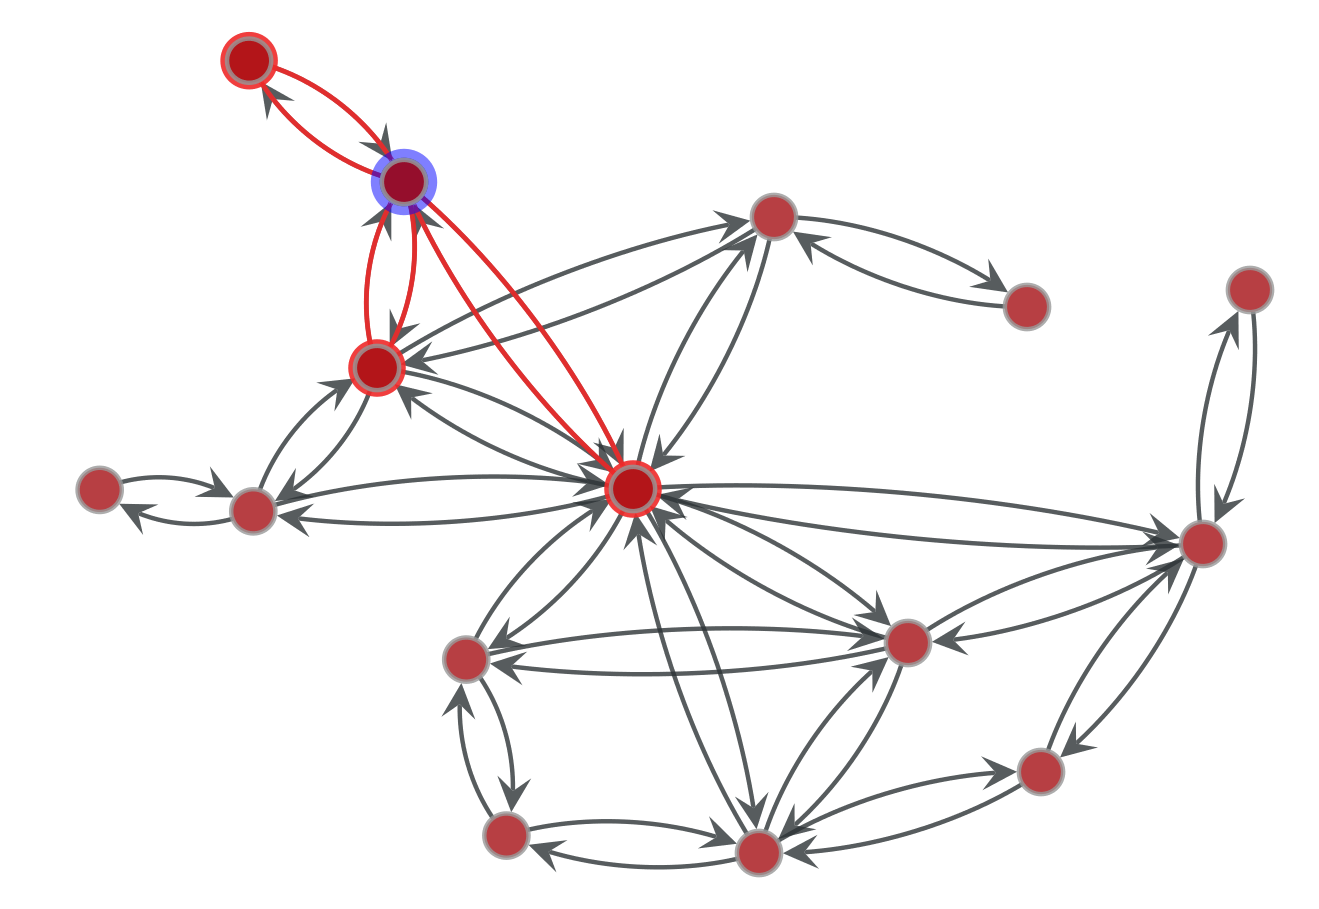
\includegraphics[width=0.5\textwidth]{test_graph.png}
        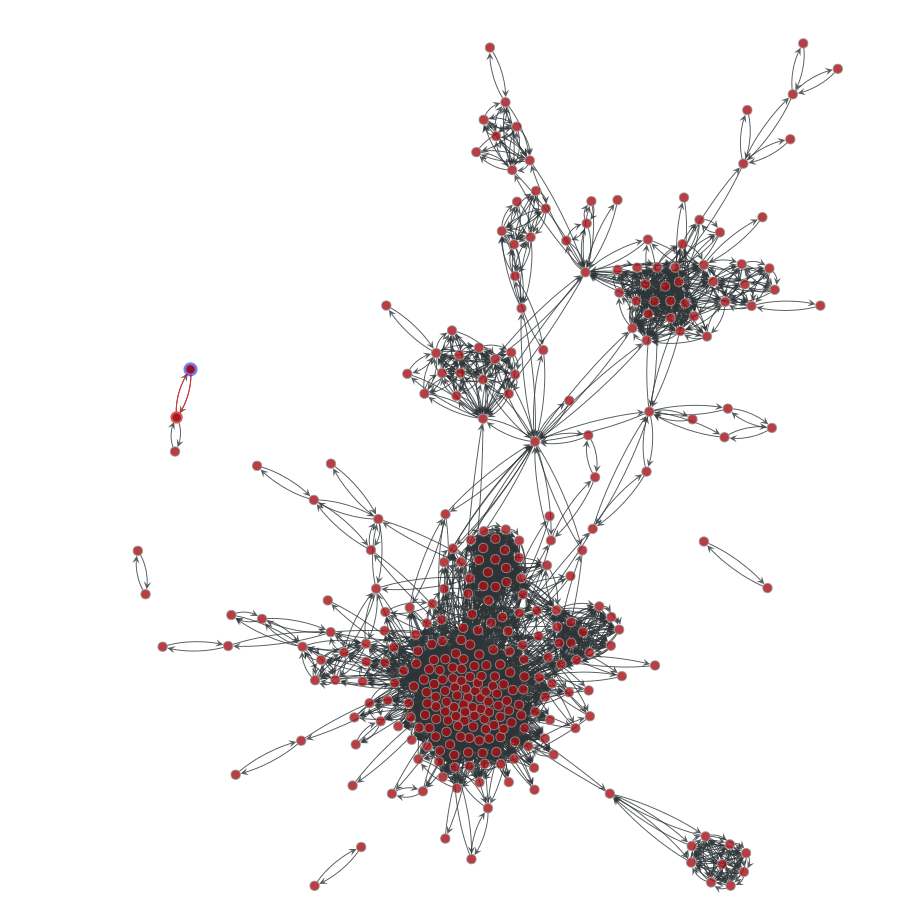
\includegraphics[width=0.5\textwidth]{facebook.png}
      \caption{SFDP force-directed layout~\cite{hu2005efficient} of our test graphs. Top: our custom test graph; bottom: facebook test graph}
        \label{fig:testgraph}
\end{figure}

 \begin{figure}
  \centering
    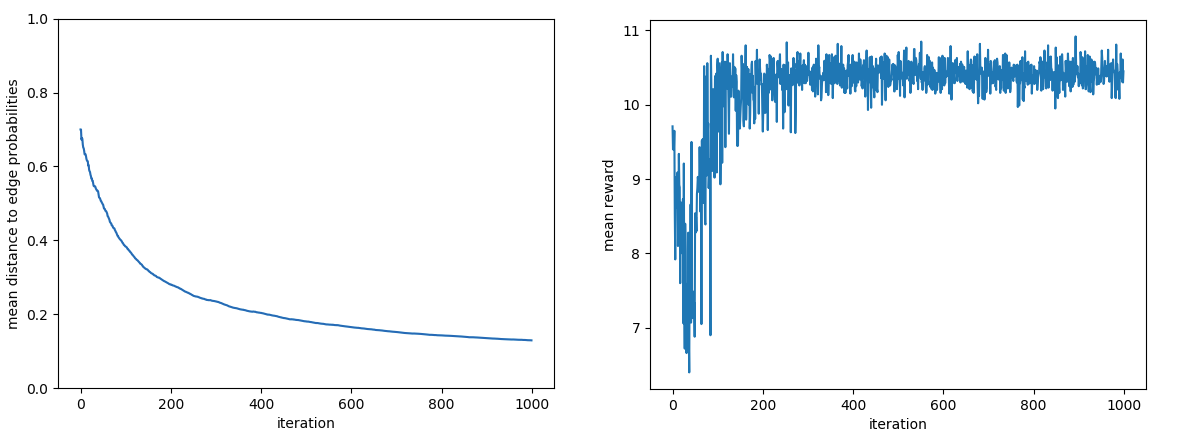
\includegraphics[width=\textwidth]{total_test.png}
      \caption{Top: our custom test graph; bottom: facebook test graph}
        \label{fig:testgraph}
\end{figure}

 \begin{figure}
  \centering
    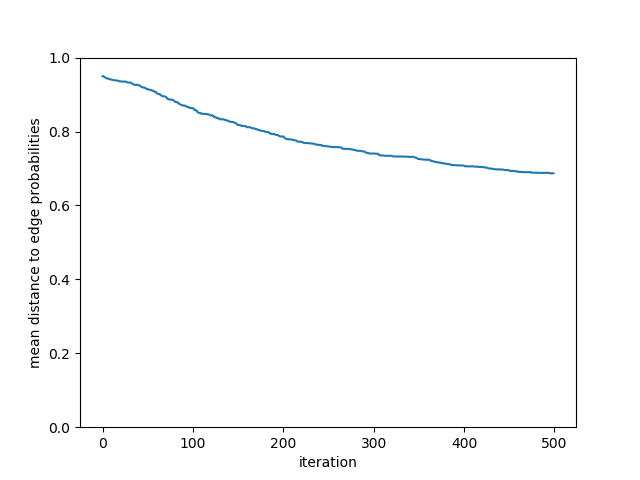
\includegraphics[width=0.5\textwidth]{conv_weights_twitter.png}
      \caption{Top: our custom test graph; bottom: facebook test graph}
        \label{fig:testgraph}
\end{figure}



\section{Conclusion}

\newpage

\bibliography{list}
\bibliographystyle{plain}

\end{document}
